% !TEX encoding = UTF-8 Unicode
\documentclass[a4paper]{article}

\usepackage{color}
\usepackage{url}
\usepackage[T2A]{fontenc} % enable Cyrillic fonts
\usepackage[utf8]{inputenc} % make weird characters work
\usepackage{graphicx}
\graphicspath{ {./images/} }
\usepackage{amsfonts}
\usepackage[english,serbian]{babel}
\usepackage{subcaption}
%\usepackage[english,serbianc]{babel} %ukljuciti babel sa ovim opcijama, umesto gornjim, ukoliko se koristi cirilica

\usepackage[unicode]{hyperref}
\hypersetup{colorlinks,citecolor=green,filecolor=green,linkcolor=blue,urlcolor=blue}

\usepackage{listings}
\usepackage{mathtools}
\usepackage{dirtytalk}
\usepackage{epigraph}
\usepackage{amssymb}


%\newtheorem{primer}{Пример}[section] %ćirilični primer
\newtheorem{primer}{Primer}[section]

\definecolor{mygreen}{rgb}{0,0.6,0}
\definecolor{mygray}{rgb}{0.5,0.5,0.5}
\definecolor{mymauve}{rgb}{0.58,0,0.82}

\lstset{ 
  backgroundcolor=\color{white},   % choose the background color; you must add \usepackage{color} or \usepackage{xcolor}; should come as last argument
  basicstyle=\scriptsize\ttfamily,        % the size of the fonts that are used for the code
  breakatwhitespace=false,         % sets if automatic breaks should only happen at whitespace
  breaklines=true,                 % sets automatic line breaking
  captionpos=b,                    % sets the caption-position to bottom
  commentstyle=\color{mygreen},    % comment style
  deletekeywords={...},            % if you want to delete keywords from the given language
  escapeinside={\%*}{*)},          % if you want to add LaTeX within your code
  extendedchars=true,              % lets you use non-ASCII characters; for 8-bits encodings only, does not work with UTF-8
  firstnumber=1000,                % start line enumeration with line 1000
  frame=single,	                   % adds a frame around the code
  keepspaces=true,                 % keeps spaces in text, useful for keeping indentation of code (possibly needs columns=flexible)
  keywordstyle=\color{blue},       % keyword style
  language=Python,                 % the language of the code
  morekeywords={*,...},            % if you want to add more keywords to the set
  numbers=left,                    % where to put the line-numbers; possible values are (none, left, right)
  numbersep=5pt,                   % how far the line-numbers are from the code
  numberstyle=\tiny\color{mygray}, % the style that is used for the line-numbers
  rulecolor=\color{black},         % if not set, the frame-color may be changed on line-breaks within not-black text (e.g. comments (green here))
  showspaces=false,                % show spaces everywhere adding particular underscores; it overrides 'showstringspaces'
  showstringspaces=false,          % underline spaces within strings only
  showtabs=false,                  % show tabs within strings adding particular underscores
  stepnumber=2,                    % the step between two line-numbers. If it's 1, each line will be numbered
  stringstyle=\color{mymauve},     % string literal style
  tabsize=2,	                   % sets default tabsize to 2 spaces
  title=\lstname                   % show the filename of files included with \lstinputlisting; also try caption instead of title
}

\begin{document}

\title{Genetski algoritam za rešavanje Sudoku-a\\
\vspace{5mm}
\small{Seminarski rad u okviru kursa\\Računarska inteligencija\\ Matematički fakultet}}

\author{Ana Miloradović, Stefan Jaćović\protect\\
\small{\texttt{ana.miloradovic7@gmail.com},} \texttt{stefanjacovic25@gmail.com}}

%\date{9.~april 2015.}


\maketitle

\abstract{
U okviru ovog rada predstavljen je primer implementacije genetskog algoritma za rešavanje popularne logičke igre Sudoku. Takođe, dat je i primer implementacije rešenja tehnikom backtracking i napravljena je analiza učinka obe tehnike. Obe tehnike implementirane su korišćenjem Python3.
}

\tableofcontents

\newpage

\section{Uvod}
\label{sec:sudoku}

\textbf{Sudoku} je popularna logička slagalica čija je pojava prvi put zabeležena  1892. godine i njen izgled je bio dosta drugačiji nego danas. Naime, današnji izgled sudokua je zasluga mnogobrojnih modifikacija iz prošlosti, pa je tako ova igra ranije podrazumevala polje koje je imalo samo četiri kvadrata, a ne devet kao što je slučaj danas.\\
Činjenica da igru mogu igrati ljudi širom sveta- bez obzira na jezik, jer su brojevi, slova i pravila svuda ista, donela je ovoj igri svetsku popularnost. Danas, gotovo da ne postoji osoba na svetu koja nije čula za ovu igru. 

\subsection{Nastanak i poreklo igre Sudoku}
Čuveni švajcarski matematičar \textbf{Leonhard Euler} sačionio je tzv. Latinski kvadrat , koji se sastojao od NxN polja obeleženih sa N različitih simbola tako da se svaki simbol u svakom redu i svakoj koloni samo jedanput ponavlja. Koristeći ovaj koncept, 1979.godine na Manhattan-u (New York), američki časopis \textbf{“Dell Math Puzzles \& Logic Problems”}, koji je inače objavljivao razne ukrštenice i zagonetke, je po prvi put objavio kvadratnu slagalicu dimenzija 9x9, koja se sastoji od 9 manjih kvadrata dimenzija 3x3, tj. upravo ono što danas nazivamo Sudoku. \\
Popularno ime koje ova slagalica nosi, osmislili su Japanci kao skraćenicu fraze “Suuji wa dokushin ni kagiru”, što grubo prevedeno znači “brojevi moraju ostati jedinstveni”. Iako ime potiče iz Japana, ova logička igra ima potiče iz \textbf{Evrope i Amerike}.\\
Sredinom osamdesetih godina prošlog veka Sudoku doživljava pravi prodor u \textbf{Japanu}, kada je prvi put objavljena u njihovom poznatom časopisu “Nikoli”. Novozelanđanin Wayne Gould je na svom putovanju po Japanu naučio da igra Sudoku, oduševio se njom, i narednih nekoliko godina razvijao kompjuterski program za generisanje ovih slagalica. Krajem 2004. godine uspeo je da ubedi londonske novine “The Times” da koristeći njegov program štampa dnevne Sudoku slagalice. Ubrzo su i druge britanske novine počele da štampaju svoje Sudoku slagalice. Igra je postala jako popularna, ne samo u Engleskoj, vec i u drugim zemljama: Nemačkoj, Austriji, SAD-u,…


\subsection{Pravila igre}
Pravila igre su vrlo jednostavna, iako rešenje često nije. Slagalicu čini kvadrat. Broj polja je najčešće 81 ($9\times9$), koji je podeljen na manje kvadrate (podkvadrate) dimenzija $3\times3$ polja. Kao početni „tragovi“, u nekoliko polja su unešene cifre, a cilj igre je da se ostala prazna polja popune tako da na kraju svaki red, kolona i podkvadrat sadrze cifre od 1 do 9 samo jedanput.\\ Sudoku slagalice su u zavisnosti od težine uglavnom podeljene na \textbf{„lake“}, \textbf{„srednje“} i \textbf{„teške“} . Treba naglasiti da težinu slagalice ne određuje samo broj unapred datih cifara, već i njihov razmeštaj u kvadratu.\\
Sudoku slagalica po pravilu ima samo \textbf{jedno moguće rešenje} (može ih imati više u slučaju da je na početku otkriven mali broj polja). U međuvremenu su se pojavile i slagalice sa $16\times16$ polja kao i druge još komplikovanije varijante, na primer kombinacija igara Sudoku i Kakuro nazvana “Killer Sudoku”. Postoji i Sudoku za decu, koji se sastoji od malog broja polja.

\begin{figure}[h]

\begin{subfigure}{0.5\textwidth}
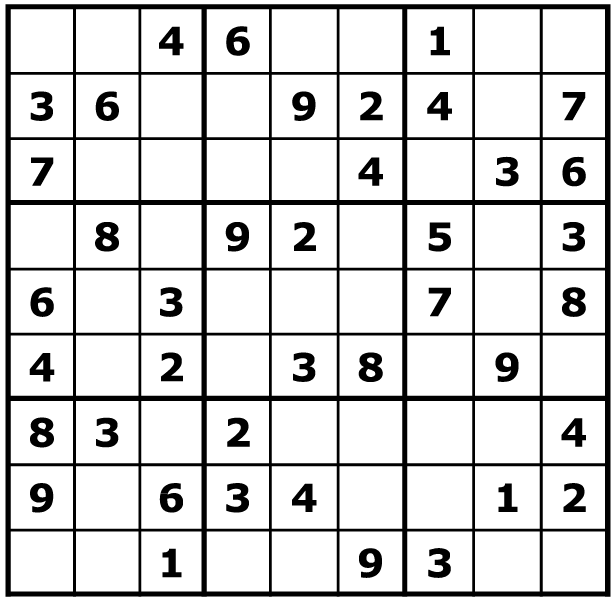
\includegraphics[width=0.8\linewidth, height=5cm]{primer_sudoku_neresen.png} 
\caption{Početna Sudoku postavka}
\label{fig:subim1}
\end{subfigure}
\begin{subfigure}{0.5\textwidth}
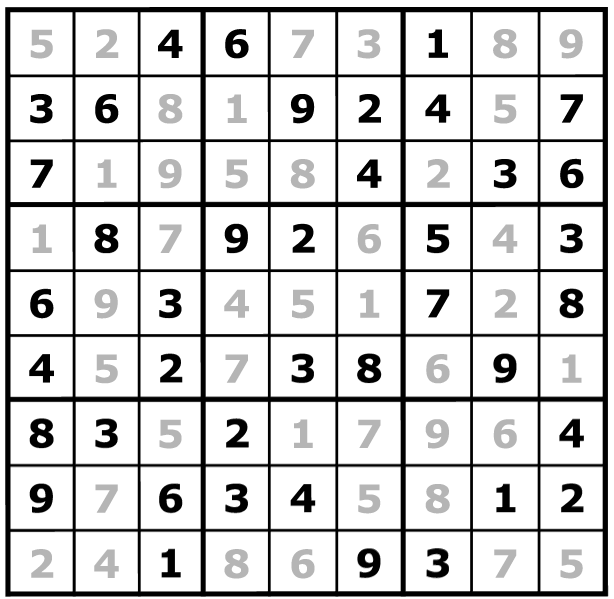
\includegraphics[width=0.8\linewidth, height=5cm]{primer_sudoku_resen.png}
\caption{Rešena Sudoku slagalica}
\label{fig:subim2}
\end{subfigure}

\caption{Primer slagalice Sudoku}
\label{fig:image2}
\end{figure}

\subsection{Sudoku i algoritmi}
Činjenica da niko ne zna algoritam kojim se uvek dolazi do rešenja bez prethodnog isprobavanja ogromnog broja kombinacija stavlja Sudoku u klasu tzv. NP-potpunih problema. Za rešavanje ove igre mogu se koristiti razni algoritmi, među kojima prednjači \textbf{backtracking} posebno za rešavanje “težih” slagalica kao i onih dimenzija $9\times9$. Takođe, koriste se i prirodom inspirisani optimizacijski algoritmi- genetski algoritam, simulirano kaljenje, optimizacija rojem čestica itd. \textbf{Genetski algoritmi} su se pokazali kao vrlo efikasni u rešavanju NP problema, međutim za rešavanje Sudoku i nisu baš efikasni (spora konvergencija, nemogućnost izlaska iz lokalnih minimuma ...)


\subsection{Genetski algoritam}
\vspace{5mm} 
\begin{figure}[h]
    \centering
    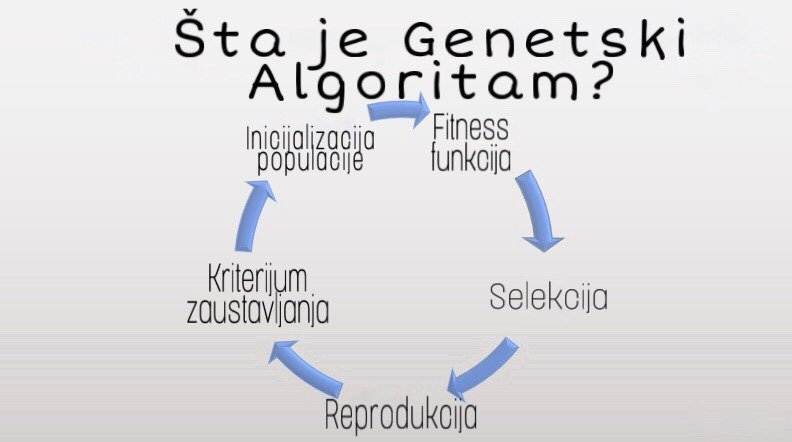
\includegraphics[scale=0.36]{GA.jpg}
    \caption{Faze genetskog algoritma}
    \label{fig:genetic algorithm}
\end{figure}
\\
\textbf{Genetski algoritam} je pretraživačka optimimizaciona tehnika, zasnovana na principima genetike i prirodne selekcije. Pripada većoj klasi evolucionih algoritama. Koristi se da se nađu optimalna ili priblizno-optimalna rešenja za teške probleme. Često se koristi za rešavanje optimizacionih problema, u istraživanjima i u mašinskom učenju. \\

\subsection{Faze genetskog algoritma}
\vspace{5mm} 
Na prethodnoj fotografiji imamo slikoviti prikaz faza genetskog algoritma. One su:
\begin{enumerate}
	\item \textbf{Inicijalizacija populacije (kodiranje):}
	\begin{itemize}
	    \item Svaki \textbf{gen} predstavlja parametar u okviru rešenja.
        \item Ovaj skup parametara koji formira rešenje naziva se \textbf{hromozom}.
        \item \textbf{Populacija} je kolekcija hromozoma.
        \item Redosled gena u hromozomu je bitan.
        \item Uglavnom, hromozomi su prikazani u binarnim formatima kao 0 i 1, ali moguća su i drugačija kodiranja.
    \end{itemize}
    
\begin{figure}[h]
    \centering
    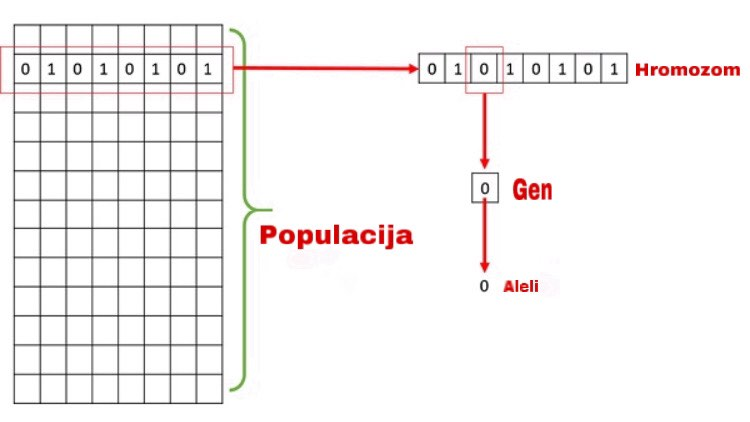
\includegraphics[scale=0.3]{oznake.jpg}
    \caption{Osnovni pojmovi GA}
    \label{fig:parts}
\end{figure}
	     
    \item \textbf{Funkcija fitnesa:}
    \begin{itemize}
	    \item Od raspoloživih hromozoma moramo odabrati one koji su najbolji za reprodukciju potomka, tako da se svakom hromozomu daje fitnes vrednost .
        \item Fitness vrednost pomaže u odabiru pojedinaca koji će se koristiti za reprodukciju.
        \item  Funkcija za fitnes je definisana u genetskoj reprezentaciji i meri kvalitet predstavljenog rešenja i ona uvek zavisi od problema.
        \item U nekim slučajevima, teško je ili nemoguće odredititi fitnes. 
    \end{itemize}
     
    \item \textbf{Selekcija:}
    \begin{itemize}
	    \item Tokom svake sledeće generacije deo postojeće populacije je izabran da odgoji novu generaciju.
        \item  Individualna rešenja su izabrana pomoču procesa baziranog na fitnesu(zdravlju), gde više fit(zdravija, sa boljom kondicijom) rešenja(merena fitnes funkcijom) imaju veće šanse da budu izabrana. Određene metode selekcije ocenjuju kondiciju svakog rešenja i prvenstveno će izabrati najbolja rešenja.
        \item U procesu selekcije, bira se hromozom za reprodukciju.
    \end{itemize}

    \item \textbf{Reprodukcija:}
    Pravljenje potomstva se dešava na dva načina: \textbf{Ukrštanjem} i \textbf{Mutacijom}
        \begin{enumerate}
             \item Ukrštanje je najbitnija faza u genetskom algoritmu. Tokom crossover-a, bira se slučajna tačka i onda se ukršta par roditelja kako bi nastali potomci. Postoje 3 glavne vrste ukrštanja:
            \begin{enumerate}
                \item \textbf{Jednopoziciono ukrštanje:} Tačka na hromozomima oba roditelja bira se nasumično i označava se kao „crossover tačka“. Bitovi desno od te tačke razmenjuju se između dva matična hromozoma. 
                \item \textbf{Dvopoziciono ukrštanje:}Dve tačke ukrštanja izabrane su nasumično iz roditeljskih hromozoma. Bitovi između dve tačke se menjaju između roditelja
                \item \textbf{Uniformno ukrštanje:} U uniformnom ukrštanju, obično se svaki bit bira između bilo kog roditelja s jednakom verovatnoćom. 
            \end{enumerate}
        Na kraju ukrštanja novo potomstvo se dodaje populaciji.
        
            \item \textbf{Mutacija:}
            U nekoliko formiranih novih potomaka, neki od njihovih gena mogu se podvrgnuti mutacijama uz malu slučajnu verovatnoću. Ovo ukazuje da se neki bitovi u hromozomu mogu okrenuti. Mutacije se rade da bi se održala raznolikosti populacije i da bi se sprečila preuranjena konvergencija. 
        \end{enumerate}
      
    \item \textbf{Konvergencija (kriterijum zaustavljanja):}\\
    Nekoliko pravila koja slede govore o tome kada se treba zaustaviti:
    \begin{itemize}
	    \item Kada ne dođe do poboljšanja kvaliteta rešenja nakon završetka određenog broja generacija zadatih unapred. 
        \item  Broj generacija je dostigao maksimalan broj generacija.
        \item Sličnost između jedinki u okviru jedne generacije je prevelika.
        \item Kada se dobije prihvatljivo rešenje.

    \end{itemize}
\end{enumerate}

\subsection{Prednosti i mane genetskog algoritma}
\renewcommand\labelitemii{$\square$}
\begin{itemize}
   \item \textbf{Prednosti GA:}
        \begin{itemize}
             \item Ne zahteva nikakve derivatne informacije (koje možda nisu dostupne za mnoge probleme u stvarnom svetu).
             \item Brži je i efikasniji u poređenju sa tradicionalnim metodama. 
             \item Ima vrlo dobre paralelne mogućnosti.
             \item Optimizira i kontinuirane i diskretne funkcije, kao i više objektivne probleme. 
             \item Pruža listu „dobrih“ rešenja, a ne samo jedno rešenje. 
             \item Uvek dobije odgovor na problem koji se vremenom popravlja. 
             \item Korisno kada je prostor za pretragu veoma velik i ako je uključen veliki broj  ‘ parametara. 
        \end{itemize}
   \item \textbf{Mane GA:}
        \begin{itemize}
             \item Nisu pogodni za sve probleme, posebno probleme koji su jednostavni i za koje su izvedene informacije o derivatima. 
             \item Vrednost fitnesa izračunava se više puta, što može biti skupo. 
             \item Budući da je stohastičan, nema garancija za optimalnost ili kvalitet rešenja.
             \item Ako se ne sprovede pravilno, GA se možda neće približiti optimalnom rešenju.
        \end{itemize}
   
\end{itemize}




\addcontentsline{toc}{section}{Literatura}
\appendix
\bibliography{bibliografija.bib} 
\bibliographystyle{plain}


\end{document}
